\subsection{飽和ドリフト速度}
半導体内に電界が印加されると、電子は電界による力を受けて加速される。この電界による速度成分のことをドリフト速度と呼ぶ。
図\ref{fg:drift} にシリコン中のドリフト速度の電界依存性を示す。横軸が電界の強さで縦軸がドリフト速度
低電界ではドリフト速度は電界に比例するが、電界が大きくなると、徐々にドリフト速度の増加割合が小さくなる。
そして、十分に高い電界になると、電荷キャリアと半導体格子との相互作用により、速度の増加が妨げられるため、ドリフト速度は飽和状態に近づく。その時の速度を飽和ドリフト速度という。
生成された電子の速度を大きくすることで、検出器の電極に誘起される信号の立ち上がりを速くすることができる。
LGAD検出器では、印加する電圧を調整することで、電子が飽和ドリフト速度に達するほどの高電場を形成することができる。
そのため、信号の立ち上がりが速くなり、優れた時間分解能を実現することが可能である。

\begin{figure}[h]
    \centering
    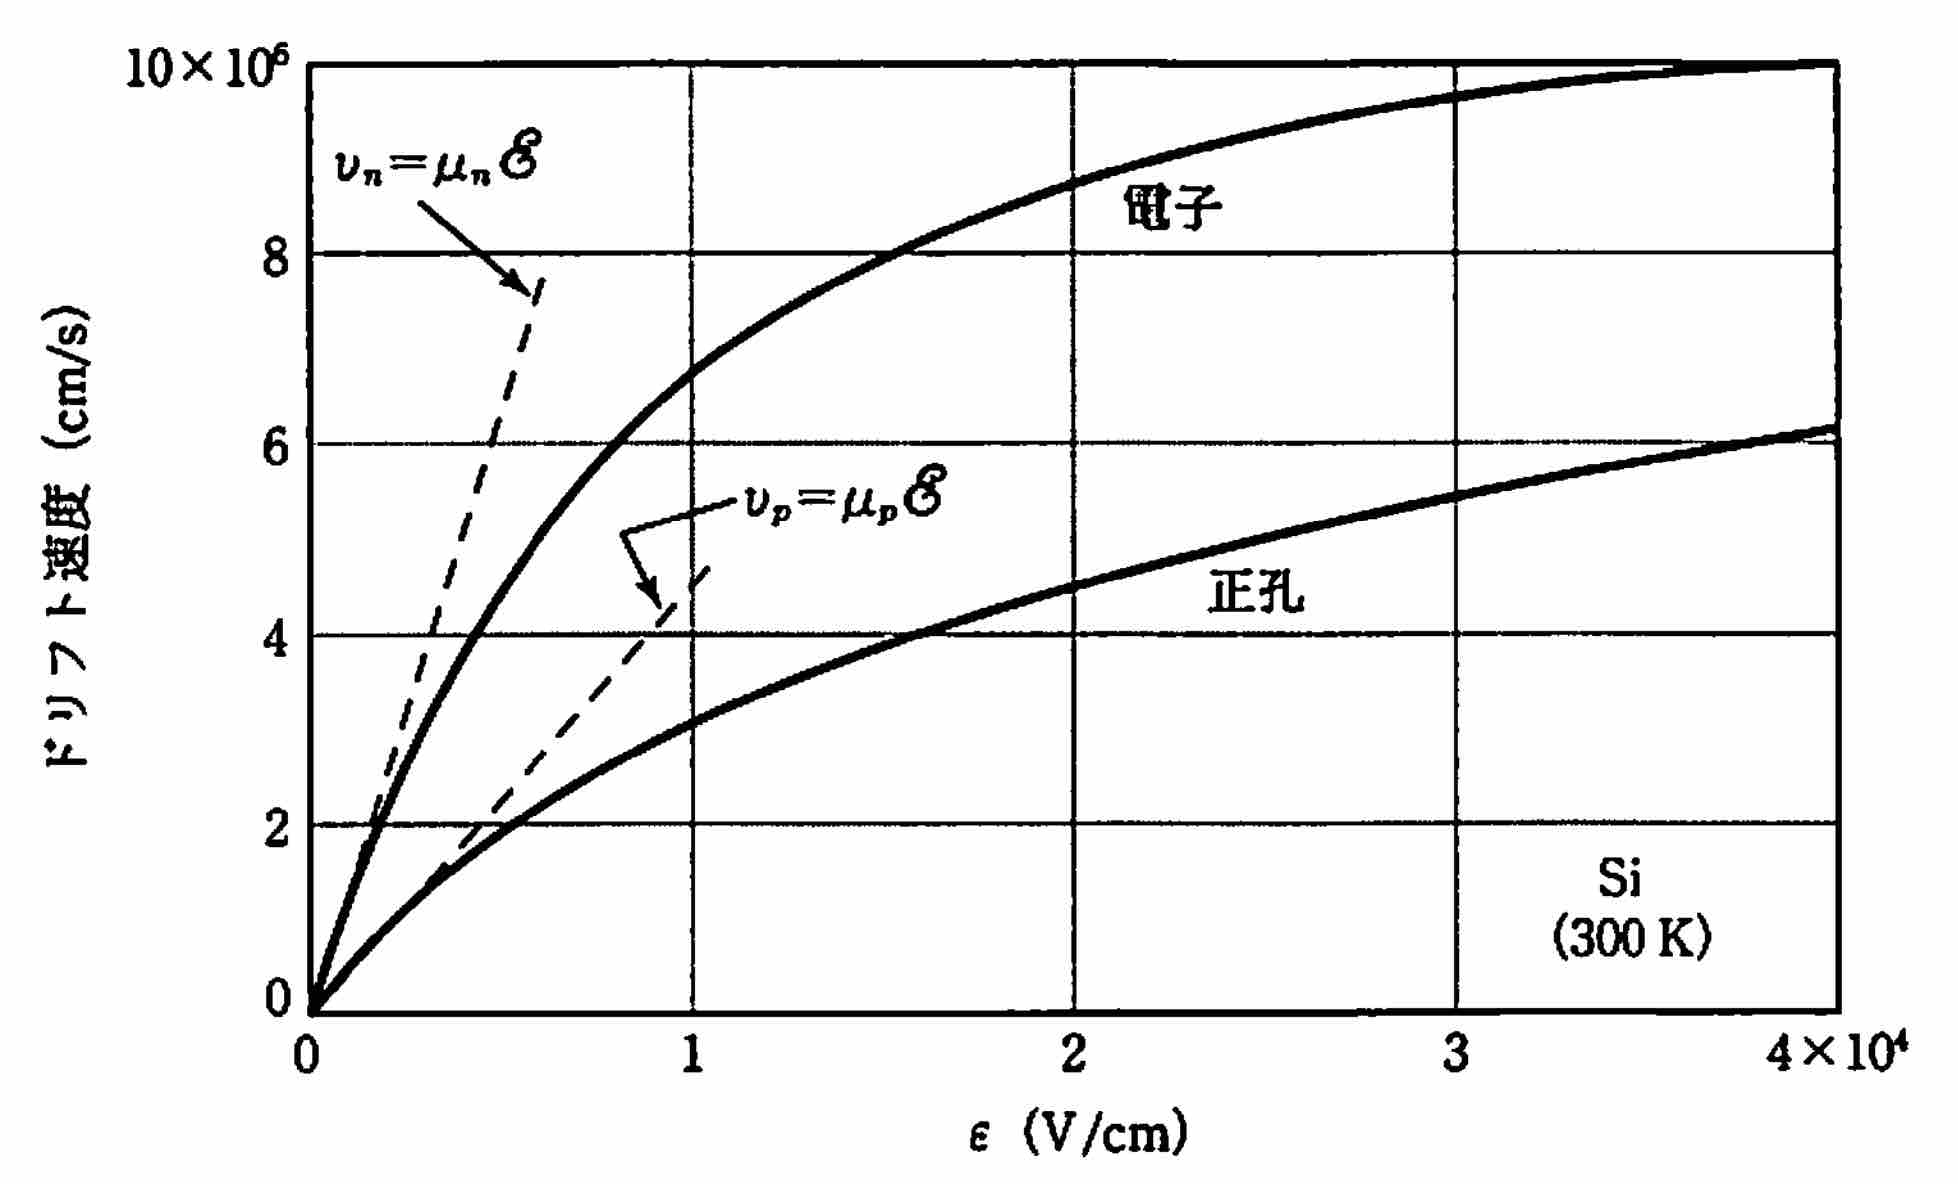
\includegraphics[width=8cm]{fig/ch3/drift.jpg}
    \caption[Si中のドリフト速度の電界依存性\cite{sze2012semiconductor}]{Si中のドリフト速度の電界依存性\cite{sze2012semiconductor}、横軸が電界の強さで縦軸がドリフト速度\\電界が強くなるとドリフト速度は増加するが、その増加割合は徐々に小さくなり飽和ドリフト速度になる。}
    \label{fg:drift}
\end{figure}

